
\documentclass[12pt,a4paper]{article}
\usepackage[utf8]{inputenc}
\usepackage[T1]{fontenc}
\usepackage{geometry}
\usepackage{times}
\usepackage{amsmath}
\usepackage{amsfonts}
\usepackage{amssymb}
\usepackage{graphicx}
\usepackage{booktabs}
\usepackage{array}
\usepackage{longtable}
\usepackage{hyperref}
\usepackage{xcolor}
\usepackage{enumitem}
\usepackage{fancyhdr}
\usepackage{listings}
\usepackage{algorithm}
\usepackage{algorithmic}
\usepackage{tikz}
\usetikzlibrary{positioning}
\usepackage{pgfplots}
\usepackage{subcaption}
\usepackage{float}

% Page geometry
\geometry{margin=1in}

% Header and footer
\pagestyle{fancy}
\fancyhf{}
\rhead{MVSEC Anomaly Detection - Technical Guide}
\lhead{Neuromorphic Event Processing}
\cfoot{\thepage}

% Colors
\definecolor{kthblue}{RGB}{25,84,166}
\definecolor{darkgray}{RGB}{64,64,64}
\definecolor{lightgray}{RGB}{240,240,240}
\definecolor{codegreen}{RGB}{0,128,0}
\definecolor{codepurple}{RGB}{163,21,132}

% Code listing style
\lstdefinestyle{pythonstyle}{
    language=Python,
    backgroundcolor=\color{lightgray},
    commentstyle=\color{codegreen},
    keywordstyle=\color{kthblue},
    numberstyle=\tiny\color{darkgray},
    stringstyle=\color{codepurple},
    basicstyle=\ttfamily\footnotesize,
    breakatwhitespace=false,
    breaklines=true,
    captionpos=b,
    keepspaces=true,
    numbers=left,
    numbersep=5pt,
    showspaces=false,
    showstringspaces=false,
    showtabs=false,
    tabsize=2,
    frame=single,
    rulecolor=\color{darkgray}
}

\lstset{style=pythonstyle}

% Title formatting
\title{\textbf{\Huge MVSEC Neuromorphic Anomaly Detection} \\ \vspace{0.5cm} \textbf{\Large Complete Technical Implementation Guide} \\ \vspace{0.3cm} \textit{A Software Engineer's Guide to Event-Based Computer Vision}}
\author{Technical Documentation \\ Based on Multi-Architecture Anomaly Detection System}
\date{\today}

% Hyperref setup
\hypersetup{
    colorlinks=true,
    linkcolor=kthblue,
    filecolor=magenta,
    urlcolor=cyan,
    citecolor=kthblue,
    pdftitle={MVSEC Anomaly Detection Technical Guide},
    pdfauthor={Technical Documentation}
}

\begin{document}

\maketitle
\tableofcontents
\newpage

\section{Executive Summary}

This technical guide provides a comprehensive overview of a neuromorphic anomaly detection system that compares three neural network architectures: Spiking Neural Networks (SNN), Recurrent Neural Networks (RNN), and Temporal Convolutional Networks (TCN). The system processes real-world event-based data from DAVIS cameras in the MVSEC dataset and employs supervised learning with systematic anomaly injection.

\subsection{How to Execute This System}

\textbf{Main Execution Point:} The entire system is orchestrated through the \texttt{run\_mvsec\_anomaly\_detection\_pipeline()} function located in the final section of the main Jupyter notebook (\texttt{notebooks/anomaly\_detection.ipynb}).

\begin{lstlisting}[caption={Primary Execution Command}]
# To run the complete system, execute this cell in the notebook:
results = run_mvsec_anomaly_detection_pipeline(
    data_path='./data',           # Path to your MVSEC dataset
    sequence='indoor_flying',     # Which MVSEC sequence to use
    camera='left',               # Camera selection (left/right)
    sensor_size=(64, 64),        # Processing resolution
    num_frames=50,               # Temporal sequence length
    max_events=500000,           # Memory management limit
    anomaly_ratio=0.5,           # 50% normal, 50% anomalous
    batch_size=8,                # Training batch size
    num_epochs=3,                # Training duration
    device='cpu'                 # Processing device
)
\end{lstlisting}

\textbf{Why This Function Exists:} This orchestrator function ties together all components of the system, providing a single entry point that handles the entire machine learning pipeline from raw data to trained models and evaluation metrics. It's designed for both research experimentation and production deployment.

\subsection{Key Technical Achievements}

\begin{itemize}
    \item \textbf{Multi-Architecture Comparison}: Implementation of SNN, RNN, and TCN for event-based anomaly detection
    \item \textbf{Real-World Data Processing}: Native MVSEC dataset integration with HDF5 file handling
    \item \textbf{Systematic Anomaly Generation}: Three distinct anomaly types with balanced dataset creation
    \item \textbf{Production-Ready Pipeline}: Complete system from raw event streams to trained models
    \item \textbf{Comprehensive Evaluation}: Multi-metric performance analysis with ROC curves and confusion matrices
\end{itemize}

\subsection{Target Audience}

This guide is designed for software engineers who want to understand:
\begin{itemize}
    \item Event-based computer vision fundamentals
    \item Neural network architecture design for temporal data
    \item Anomaly detection in sparse, asynchronous data streams
    \item Production-level machine learning pipeline implementation
\end{itemize}

\section{System Architecture Overview}

\subsection{High-Level Architecture}

The system follows a modular pipeline architecture that separates concerns and enables easy extension:

\begin{figure}[H]
\centering
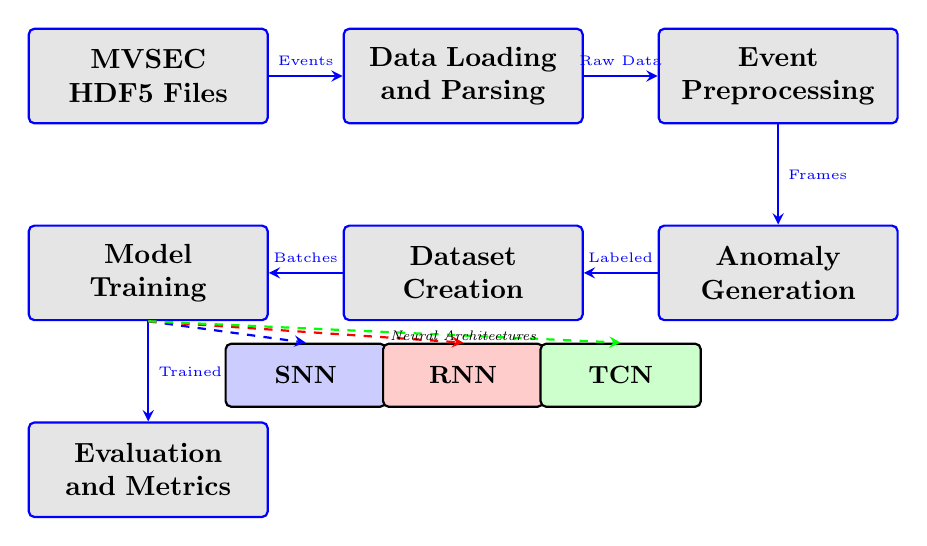
\begin{tikzpicture}[
    node distance=2.5cm and 3cm,
    block/.style={rectangle, draw=blue, thick, fill=gray!20, text width=2.8cm, text centered, minimum height=1.2cm, rounded corners=2pt},
    archblock/.style={rectangle, draw=black, thick, text width=1.8cm, text centered, minimum height=0.8cm, rounded corners=2pt, font=\small\bfseries},
    arrow/.style={thick,->,>=stealth, color=blue}
]

% Define main pipeline nodes
\node [block] (data) at (0,0) {\textbf{MVSEC} \\ \textbf{HDF5 Files}};
\node [block] (load) at (4,0) {\textbf{Data Loading} \\ \textbf{and Parsing}};
\node [block] (preprocess) at (8,0) {\textbf{Event} \\ \textbf{Preprocessing}};
\node [block] (anomaly) at (8,-2.5) {\textbf{Anomaly} \\ \textbf{Generation}};
\node [block] (dataset) at (4,-2.5) {\textbf{Dataset} \\ \textbf{Creation}};
\node [block] (models) at (0,-2.5) {\textbf{Model} \\ \textbf{Training}};
\node [block] (eval) at (0,-5) {\textbf{Evaluation} \\ \textbf{and Metrics}};

% Draw main pipeline arrows with labels
\draw [arrow] (data) -- (load) node[midway, above, font=\tiny] {Events};
\draw [arrow] (load) -- (preprocess) node[midway, above, font=\tiny] {Raw Data};
\draw [arrow] (preprocess) -- (anomaly) node[midway, right, font=\tiny] {Frames};
\draw [arrow] (anomaly) -- (dataset) node[midway, above, font=\tiny] {Labeled};
\draw [arrow] (dataset) -- (models) node[midway, above, font=\tiny] {Batches};
\draw [arrow] (models) -- (eval) node[midway, right, font=\tiny] {Trained Models};

% Add architecture boxes horizontally aligned
\node [archblock, fill=blue!20] (snn) at (2,-3.8) {\textbf{SNN}};
\node [archblock, fill=red!20] (rnn) at (4,-3.8) {\textbf{RNN}};
\node [archblock, fill=green!20] (tcn) at (6,-3.8) {\textbf{TCN}};

% Connect models to architectures with simple arrows
\draw [arrow, dashed, color=blue] (models.south) -- (snn.north);
\draw [arrow, dashed, color=red] (models.south) -- (rnn.north);
\draw [arrow, dashed, color=green] (models.south) -- (tcn.north);

% Add architecture label
\node at (4,-3.3) [font=\tiny\itshape] {Neural Architectures};

\end{tikzpicture}
\caption{System Architecture Pipeline - Complete Data Flow from MVSEC Files to Model Evaluation}
\end{figure}

\subsection{Core Components}

\begin{enumerate}
    \item \textbf{Data Pipeline}: MVSEC dataset loading, event parsing, temporal binning
    \item \textbf{Anomaly Generator}: Systematic injection of realistic failure modes
    \item \textbf{Neural Architectures}: Three distinct approaches to temporal modeling
    \item \textbf{Training Framework}: Supervised learning with comprehensive metrics
    \item \textbf{Evaluation System}: Performance comparison and visualization
\end{enumerate}

\section{Understanding Event-Based Vision}

\subsection{What Are Event Cameras?}

Event cameras (Dynamic Vision Sensors) represent a paradigm shift from traditional frame-based imaging:

\begin{table}[H]
\centering
\begin{tabular}{|l|l|l|}
\hline
\textbf{Aspect} & \textbf{Traditional Camera} & \textbf{Event Camera} \\
\hline
Data Capture & Fixed frame rate (30 FPS) & Asynchronous events \\
Temporal Resolution & 33ms between frames & Microsecond precision \\
Data Volume & Dense frames (megapixels) & Sparse events (thousands) \\
Power Consumption & High (continuous capture) & Low (change-driven) \\
Dynamic Range & Limited & Very high (140dB) \\
Motion Blur & Present in fast motion & None \\
\hline
\end{tabular}
\caption{Event vs Traditional Camera Comparison}
\end{table}

\subsection{Event Data Structure}

Each event is represented as a 4-tuple:
\begin{align}
\text{Event} = (x, y, t, p)
\end{align}

Where:
\begin{itemize}
    \item $x, y$: Spatial coordinates (pixel location)
    \item $t$: Timestamp (microsecond precision)
    \item $p$: Polarity ($+1$ for brightness increase, $-1$ for decrease)
\end{itemize}

\subsection{Why Event-Based Anomaly Detection?}

Event cameras are ideal for anomaly detection because:
\begin{itemize}
    \item \textbf{High Temporal Resolution}: Captures fast anomalies that frame cameras miss
    \item \textbf{Low Latency}: Real-time processing capabilities
    \item \textbf{Robust to Lighting}: Works in challenging illumination conditions
    \item \textbf{Sparse Data}: Natural focus on changing regions (where anomalies occur)
\end{itemize}

\section{Data Pipeline Implementation}

\subsection{MVSEC Dataset Integration}

The Multi-Vehicle Stereo Event Camera (MVSEC) dataset provides real-world event data from aerial navigation scenarios.

\subsubsection{Dataset Characteristics}

\begin{itemize}
    \item \textbf{Sensor}: DAVIS 346B cameras (260×346 resolution)
    \item \textbf{Scenarios}: Indoor/outdoor flying sequences
    \item \textbf{Data Volume}: ~24 million events per sequence
    \item \textbf{Format}: HDF5 files with hierarchical structure
\end{itemize}

\subsubsection{HDF5 File Structure}

\textbf{Purpose:} MVSEC data is stored in HDF5 format, which is a hierarchical data format optimized for large scientific datasets. Understanding this structure is crucial for accessing the raw event data.

\textbf{Usage Context:} This function is called during the data loading phase of the pipeline. It's the foundation that enables everything else - without proper data loading, the entire system cannot function.

\textbf{Why HDF5?} Event cameras generate millions of events per second. HDF5 provides efficient storage and random access to these large datasets, making it the standard format for neuromorphic data.

\begin{lstlisting}[caption={MVSEC HDF5 File Navigation - Core Data Access Function}]
# HDF5 file structure:
# /davis/left/events    - Left camera event data
# /davis/right/events   - Right camera event data
# Each event: [x, y, timestamp, polarity]

def load_mvsec_data(data_path, sequence='indoor_flying', camera='left'):
    """
    Load MVSEC dataset from HDF5 files

    Args:
        data_path: Path to MVSEC data directory
        sequence: Which sequence to use
        camera: Which camera ('left' or 'right')

    Returns:
        events: Dictionary with event data (x, y, t, p)
        sensor_size: Camera resolution tuple
    """
    with h5py.File(data_file, 'r') as f:
        # Navigate to camera events
        events_data = f['davis'][camera]['events'][:]

        # Extract event components
        events = {
            'x': events_data[:, 0].astype(int),
            'y': events_data[:, 1].astype(int),
            't': events_data[:, 2],
            'p': events_data[:, 3].astype(int)
        }

        return events, (260, 346)  # DAVIS 346B resolution
\end{lstlisting}

\subsection{Event Preprocessing Pipeline}

\subsubsection{Temporal Binning Strategy}

\textbf{The Challenge:} Event cameras produce asynchronous, sparse data streams that neural networks cannot directly process. Traditional CNNs expect dense, synchronous image frames.

\textbf{Our Solution:} Temporal binning converts continuous event streams into discrete frame sequences that maintain temporal information while being compatible with standard neural network architectures.

\textbf{Why This Matters:} This preprocessing step is critical because it determines how temporal information is preserved and presented to the neural networks. Poor binning can lose important temporal dynamics, while good binning captures the essence of the event-based data.

Event streams are continuous and asynchronous. For neural network processing, we convert them to discrete frame sequences:

\begin{figure}[H]
\centering
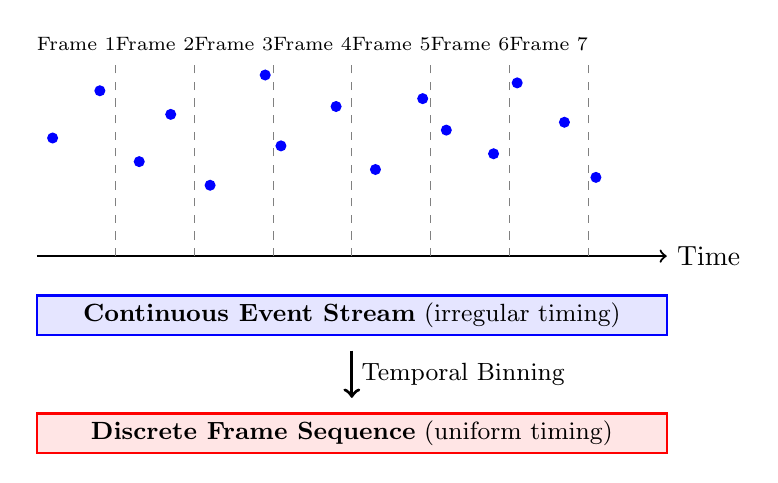
\begin{tikzpicture}[scale=1.0]
% Simple time axis
\draw[->, thick] (0,0) -- (8,0) node[right] {Time};

% Draw time bins as vertical dashed lines
\foreach \x in {1,2,3,4,5,6,7} {
    \draw[dashed, gray] (\x,0) -- (\x,2.5);
}

% Add frame labels
\foreach \x/\label in {0.5/1, 1.5/2, 2.5/3, 3.5/4, 4.5/5, 5.5/6, 6.5/7} {
    \node at (\x,2.7) [font=\scriptsize] {Frame \label};
}

% Draw events as simple dots
\foreach \x/\y in {0.2/1.5, 0.8/2.1, 1.3/1.2, 1.7/1.8, 2.2/0.9, 2.9/2.3, 3.1/1.4, 3.8/1.9, 4.3/1.1, 4.9/2.0, 5.2/1.6, 5.8/1.3, 6.1/2.2, 6.7/1.7, 7.1/1.0} {
    \fill[blue] (\x,\y) circle (2pt);
}

% Add explanation boxes
\draw[thick, blue, fill=blue!10] (0,-1) rectangle (8,-0.5);
\node at (4,-0.75) [font=\small] {\textbf{Continuous Event Stream} (irregular timing)};

\draw[->, very thick] (4,-1.2) -- (4,-1.8);
\node at (4,-1.5) [right, font=\small] {Temporal Binning};

\draw[thick, red, fill=red!10] (0,-2.5) rectangle (8,-2);
\node at (4,-2.25) [font=\small] {\textbf{Discrete Frame Sequence} (uniform timing)};

\end{tikzpicture}
\caption{Temporal Binning Process - Converting Continuous Events to Discrete Frames}
\end{figure}

\textbf{Implementation Strategy:} This function is the heart of our preprocessing pipeline. It transforms millions of individual events into structured tensors that our neural networks can learn from.

\textbf{Key Design Decisions:}
\begin{itemize}
    \item \textbf{Dual-channel representation}: Separates positive and negative events for richer feature representation
    \item \textbf{Uniform time bins}: Ensures consistent temporal spacing for stable training
    \item \textbf{Spatial accumulation}: Multiple events in the same pixel-time bin are summed
    \item \textbf{Frame normalization}: Each frame is normalized independently to [0,1] range
\end{itemize}

\textbf{When This Runs:} Called by \texttt{MVSECDataHandler.create\_dataset()} during the data preprocessing phase, before anomaly injection.

\begin{lstlisting}[caption={Temporal Binning Implementation - Converting Events to Neural Network Input}]
def preprocess_events(self, events, num_frames=50):
    """
    Convert continuous event stream to discrete frame sequence

    Args:
        events: Event dictionary {x, y, t, p}
        num_frames: Number of frames to generate

    Returns:
        frames: Tensor (num_frames, 2, H, W)
                Channel 0: positive events
                Channel 1: negative events
    """
    x, y, t, p = events['x'], events['y'], events['t'], events['p']

    # Create uniform time bins
    t_min, t_max = np.min(t), np.max(t)
    time_bins = np.linspace(t_min, t_max, num_frames + 1)

    # Initialize frame tensor
    H, W = self.sensor_size
    frames = torch.zeros((num_frames, 2, H, W))

    # Bin events into frames
    for i in range(len(x)):
        # Find time bin
        bin_idx = np.searchsorted(time_bins[1:], t[i])
        bin_idx = min(bin_idx, num_frames - 1)

        # Map polarity to channel
        channel = 0 if p[i] == 1 else 1

        # Accumulate event
        if 0 <= y[i] < H and 0 <= x[i] < W:
            frames[bin_idx, channel, y[i], x[i]] += 1

    # Normalize frames
    for f in range(num_frames):
        for c in range(2):
            max_val = frames[f, c].max()
            if max_val > 0:
                frames[f, c] /= max_val

    return frames
\end{lstlisting}

\subsubsection{Memory Management Strategy}

\textbf{The Problem:} MVSEC sequences contain 20+ million events each. Loading and processing all events simultaneously would require 100+ GB of RAM and cause out-of-memory errors.

\textbf{Our Approach:} Implement a multi-level memory management strategy that maintains data quality while ensuring the system runs on standard hardware.

\textbf{Why Each Strategy:}
\begin{itemize}
    \item \textbf{Event Sampling (500K limit)}: Reduces memory footprint by 40x while maintaining statistical representativeness
    \item \textbf{Spatial Downsampling (260×346 → 64×64)}: Reduces spatial dimensions by 17x, enabling faster training without losing essential patterns
    \item \textbf{Small Batch Sizes (8-16)}: Prevents GPU memory overflow during training, especially important for SNN models
    \item \textbf{Progressive Loading}: Loads data on-demand rather than pre-loading entire dataset
\end{itemize}

\textbf{Trade-offs:} We sacrifice some data completeness for practical usability. In production systems, these limits can be adjusted based on available hardware.

\section{Anomaly Generation Strategy}

\subsection{Supervised Learning Approach}

Since natural anomalies in event data are rare and unlabeled, we employ systematic anomaly injection to create a balanced, labeled dataset.

\subsection{Three Core Anomaly Types}

\textbf{Design Philosophy:} Since natural anomalies in event data are rare and unlabeled, we systematically generate realistic anomalies that correspond to actual sensor failure modes. Each anomaly type is designed to test different aspects of the neural networks' pattern recognition capabilities.

\textbf{Strategic Approach:} The three anomaly types are complementary:
\begin{itemize}
    \item \textbf{Blackout}: Tests spatial pattern recognition (missing information)
    \item \textbf{Vibration}: Tests noise robustness (added information)
    \item \textbf{Polarity Flip}: Tests event-specific understanding (corrupted information)
\end{itemize}

\textbf{Balance Consideration:} 50/50 normal-to-anomalous ratio ensures the models learn to distinguish rather than simply memorizing the majority class.

\begin{table}[H]
\centering
\begin{tabular}{|p{3cm}|p{4cm}|p{4cm}|p{3cm}|}
\hline
\textbf{Anomaly Type} & \textbf{Implementation} & \textbf{Real-World Scenario} & \textbf{Parameters} \\
\hline
\textbf{Blackout Regions} & Zero out events in spatial regions & Sensor occlusion, hardware failure & 70-100\% reduction, 10-40px regions \\
\hline
\textbf{Vibration Noise} & Add Gaussian noise to localized areas & Camera shake, mechanical vibration & 0.3-0.7 intensity, 20-60px coverage \\
\hline
\textbf{Polarity Flipping} & Swap positive/negative event channels & Hardware errors, circuit malfunctions & 60-90\% flip probability, 15-45px regions \\
\hline
\end{tabular}
\caption{Anomaly Types and Motivations}
\end{table}

\subsection{Anomaly Generation Implementation}

\subsubsection{Blackout Region Anomaly}

\textbf{Real-World Motivation:} Event cameras in autonomous vehicles or drones can experience partial sensor failures, dust accumulation, or physical occlusion. This anomaly simulates these critical failure modes.

\textbf{Technical Implementation:} Multiplicatively reduces pixel intensities in random spatial regions, simulating areas where the sensor stops responding to light changes.

\textbf{Why This Design:}
\begin{itemize}
    \item \textbf{Random positioning}: Ensures models can't memorize specific locations
    \item \textbf{Variable intensity}: Tests detection at different severity levels
    \item \textbf{Rectangular regions}: Matches realistic occlusion patterns
\end{itemize}

\textbf{Integration Point:} Called by \texttt{AnomalyGenerator.add\_random\_anomaly()} during dataset creation.

\begin{lstlisting}[caption={Blackout Region Implementation - Simulating Sensor Occlusion}]
def add_blackout_region(self, frame, region_size=(20, 20), intensity=1.0):
    """
    Simulate sensor failure by zeroing out spatial region

    Args:
        frame: Input frame tensor (C, H, W)
        region_size: Size of blackout region (height, width)
        intensity: Blackout intensity (0.0-1.0)

    Returns:
        frame_with_anomaly: Modified frame
        mask: Binary mask showing anomaly location
    """
    C, H, W = frame.shape
    rh, rw = region_size

    frame_with_anomaly = frame.clone()

    # Random position
    y = self.rng.randint(0, H - rh - 1)
    x = self.rng.randint(0, W - rw - 1)

    # Create mask
    mask = torch.zeros((H, W), dtype=torch.bool)
    mask[y:y+rh, x:x+rw] = True

    # Apply blackout
    for c in range(C):
        frame_with_anomaly[c][mask] *= (1 - intensity)

    return frame_with_anomaly, mask
\end{lstlisting}

\subsubsection{Vibration Noise Anomaly}

\textbf{Real-World Scenario:} Mobile platforms (drones, vehicles) experience mechanical vibrations that can cause camera shake, leading to spurious events and motion blur in event cameras.

\textbf{Technical Approach:} Additive Gaussian noise in localized regions simulates the extra events generated by rapid, small-scale motion.

\textbf{Design Rationale:}
\begin{itemize}
    \item \textbf{Gaussian distribution}: Models natural vibration patterns
    \item \textbf{Localized regions}: Vibrations affect specific sensor areas
    \item \textbf{Intensity control}: Parameterizes severity from mild to severe
    \item \textbf{Clamping to [0,1]}: Maintains realistic pixel intensity ranges
\end{itemize}

\textbf{Testing Purpose:} Evaluates how well models distinguish signal from noise, a critical capability for real-world deployment.

\begin{lstlisting}[caption={Vibration Noise Implementation - Simulating Mechanical Disturbances}]
def add_vibration_noise(self, frame, region_size=(40, 40), intensity=0.5):
    """
    Simulate camera shake with additive Gaussian noise

    Args:
        frame: Input frame tensor (C, H, W)
        region_size: Size of vibration region
        intensity: Noise intensity

    Returns:
        frame_with_anomaly: Modified frame
        mask: Binary mask showing anomaly location
    """
    C, H, W = frame.shape
    rh, rw = region_size

    frame_with_anomaly = frame.clone()

    # Random position
    y = self.rng.randint(0, H - rh - 1)
    x = self.rng.randint(0, W - rw - 1)

    # Create mask
    mask = torch.zeros((H, W), dtype=torch.bool)
    mask[y:y+rh, x:x+rw] = True

    # Add noise
    for c in range(C):
        noise = torch.randn(rh, rw) * intensity
        frame_with_anomaly[c][y:y+rh, x:x+rw] += noise
        frame_with_anomaly[c] = torch.clamp(frame_with_anomaly[c], 0, 1)

    return frame_with_anomaly, mask
\end{lstlisting}

\subsubsection{Polarity Flipping Anomaly}

\textbf{Hardware Failure Context:} Event cameras have complex analog circuits that determine event polarity. Hardware malfunctions, electromagnetic interference, or temperature extremes can cause polarity inversion.

\textbf{Event-Specific Nature:} This anomaly is unique to event cameras and tests whether models understand the fundamental difference between positive and negative events.

\textbf{Implementation Details:}
\begin{itemize}
    \item \textbf{Channel swapping}: Positive events → negative channel, negative events → positive channel
    \item \textbf{Probabilistic flipping}: Not all pixels flip, creating realistic partial failures
    \item \textbf{Spatial localization}: Hardware failures typically affect circuit regions
\end{itemize}

\textbf{Model Testing:} This anomaly specifically tests event-based understanding - traditional computer vision models might miss this, but neuromorphic-aware models should detect it.

\begin{lstlisting}[caption={Polarity Flipping Implementation - Simulating Circuit Malfunctions}]
def flip_polarities(self, frame, region_size=(30, 30), flip_prob=0.8):
    """
    Simulate hardware errors by flipping event polarities

    Args:
        frame: Input frame tensor (2, H, W) - pos/neg channels
        region_size: Size of flip region
        flip_prob: Probability of flipping each pixel

    Returns:
        frame_with_anomaly: Modified frame
        mask: Binary mask showing anomaly location
    """
    C, H, W = frame.shape
    assert C == 2, "Polarity flipping requires 2-channel input"

    rh, rw = region_size
    frame_with_anomaly = frame.clone()

    # Random position
    y = self.rng.randint(0, H - rh - 1)
    x = self.rng.randint(0, W - rw - 1)

    # Create masks
    mask = torch.zeros((H, W), dtype=torch.bool)
    mask[y:y+rh, x:x+rw] = True
    flip_mask = torch.rand(rh, rw) < flip_prob

    # Store original values
    pos_events = frame_with_anomaly[0, y:y+rh, x:x+rw].clone()
    neg_events = frame_with_anomaly[1, y:y+rh, x:x+rw].clone()

    # Apply flipping
    frame_with_anomaly[0, y:y+rh, x:x+rw][flip_mask] = neg_events[flip_mask]
    frame_with_anomaly[1, y:y+rh, x:x+rw][flip_mask] = pos_events[flip_mask]

    return frame_with_anomaly, mask
\end{lstlisting}

\section{Neural Network Architectures}

\subsection{Architecture Comparison Overview}

\textbf{Research Question:} Which neural architecture is best suited for processing event-based data? Each architecture represents a different philosophy for handling temporal information.

\textbf{Fair Comparison Strategy:} All models receive identical preprocessed data, use the same training procedures, and are evaluated with identical metrics. This ensures architectural differences drive performance variations, not implementation details.

\textbf{Why These Three Architectures:}
\begin{itemize}
    \item \textbf{SNN}: Bio-inspired, theoretically optimal for event data
    \item \textbf{RNN}: Proven sequential processing, industry standard
    \item \textbf{TCN}: Modern parallel processing, state-of-the-art for temporal tasks
\end{itemize}

The system implements three distinct approaches to temporal sequence processing:

\begin{table}[H]
\centering
\begin{tabular}{|l|p{4cm}|p{4cm}|p{4cm}|}
\hline
\textbf{Architecture} & \textbf{Key Principle} & \textbf{Advantages} & \textbf{Challenges} \\
\hline
\textbf{SNN} & Bio-inspired spike-based computation & Energy efficient, event-native & Training complexity, surrogate gradients \\
\hline
\textbf{RNN} & Sequential memory-based processing & Proven temporal modeling & Vanishing gradients, sequential bottleneck \\
\hline
\textbf{TCN} & Parallel dilated convolutions & Long-range dependencies, parallel & Memory intensive, receptive field design \\
\hline
\end{tabular}
\caption{Neural Architecture Comparison}
\end{table}

\subsection{Spiking Neural Network (SNN) Implementation}

\subsubsection{Surrogate Gradient Method}

\textbf{The SNN Training Problem:} Spiking neurons use discrete step functions (0 or 1 outputs), which have zero gradients almost everywhere. Standard backpropagation cannot train these networks.

\textbf{Surrogate Gradient Solution:} Replace the non-differentiable step function with a smooth approximation during backpropagation while keeping the discrete spikes during forward pass.

\textbf{Why This Approach:}
\begin{itemize}
    \item \textbf{Maintains spike properties}: Forward passes use actual discrete spikes
    \item \textbf{Enables learning}: Backward passes use smooth gradients
    \item \textbf{Proven effective}: Standard method in neuromorphic computing
\end{itemize}

\textbf{Implementation Challenge:} Must balance gradient smoothness (for learning) with spike discreteness (for biological realism).

SNNs use discrete spikes, making them non-differentiable. We employ surrogate gradients for backpropagation:

\begin{lstlisting}[caption={Surrogate Gradient Implementation - Enabling SNN Training}]
class SurrogateSpike(torch.autograd.Function):
    """
    Surrogate gradient for Heaviside step function
    """
    @staticmethod
    def forward(ctx, input, alpha=10.0):
        ctx.save_for_backward(input)
        ctx.alpha = alpha
        return (input > 0).float()  # Heaviside step

    @staticmethod
    def backward(ctx, grad_output):
        input, = ctx.saved_tensors
        alpha = ctx.alpha
        # Sigmoid surrogate gradient
        grad_input = grad_output * alpha * torch.exp(-alpha * torch.abs(input)) / (1 + torch.exp(-alpha * input))**2
        return grad_input, None

surrogate_spike = SurrogateSpike.apply
\end{lstlisting}

\subsubsection{Spiking Neuron Dynamics}

\textbf{Biological Inspiration:} This implements the Leaky Integrate-and-Fire (LIF) neuron model, which mimics how real neurons accumulate input signals and fire spikes when a threshold is reached.

\textbf{Key Components:}
\begin{itemize}
    \item \textbf{Membrane potential}: Accumulates input over time
    \item \textbf{Leak factor (β)}: Causes potential to decay, preventing infinite accumulation
    \item \textbf{Threshold}: Firing threshold that triggers spikes
    \item \textbf{Reset mechanism}: How potential is reset after spiking
\end{itemize}

\textbf{Why LIF for Event Data:} Event cameras are bio-inspired sensors, so bio-inspired processing is a natural match. The temporal dynamics of LIF neurons can capture the temporal patterns in event streams.

\textbf{Usage in Pipeline:} These neurons form the core computational units in our SNN architecture, processing the temporal binned event data.

\begin{lstlisting}[caption={Spiking Neuron Implementation - LIF Neuron Dynamics}]
class SpikingNeuron(nn.Module):
    def __init__(self, beta=0.9, threshold=1.0, reset_mode='subtract'):
        """
        Leaky Integrate-and-Fire neuron model

        Args:
            beta: Membrane potential decay factor
            threshold: Spike threshold
            reset_mode: 'subtract' or 'zero' reset
        """
        super().__init__()
        self.beta = beta
        self.threshold = threshold
        self.reset_mode = reset_mode

    def forward(self, input_current, mem=None):
        """
        Neuron dynamics: V[t] = β*V[t-1] + I[t]

        Args:
            input_current: Input current at time t
            mem: Previous membrane potential

        Returns:
            spike: Output spike (0 or 1)
            mem: Updated membrane potential
        """
        if mem is None:
            mem = torch.zeros_like(input_current)

        # Update membrane potential
        mem = self.beta * mem + input_current

        # Generate spikes
        spike = surrogate_spike(mem - self.threshold)

        # Reset mechanism
        if self.reset_mode == 'subtract':
            mem = mem - spike * self.threshold
        elif self.reset_mode == 'zero':
            mem = mem * (1 - spike)

        return spike, mem
\end{lstlisting}

\subsubsection{Complete SNN Architecture}

\textbf{Architecture Philosophy:} Combines convolutional layers for spatial feature extraction with spiking dynamics for temporal processing. This hybrid approach leverages the strengths of both paradigms.

\textbf{Layer Design Rationale:}
\begin{itemize}
    \item \textbf{Progressive downsampling}: 3 conv layers with stride=2 reduce spatial dimensions
    \item \textbf{Channel expansion}: 16 → 32 → 64 channels increase feature complexity
    \item \textbf{Global pooling}: Reduces spatial dimensions to single values
    \item \textbf{Binary classification}: Final FC layer outputs normal vs anomaly scores
\end{itemize}

\textbf{Memory Management:} Membrane potentials are reset each forward pass to prevent accumulation across batches, ensuring consistent behavior.

\textbf{Training Integration:} This model is instantiated and trained by the main pipeline function, competing directly with RNN and TCN variants.

\begin{lstlisting}[caption={SNN Anomaly Detector - Complete Bio-Inspired Architecture}]
class SpikingAnomalyDetector(nn.Module):
    def __init__(self, input_channels=2, hidden_channels=16, output_dim=2):
        """
        SNN for event-based anomaly detection

        Architecture:
        - Convolutional spiking layers with downsampling
        - Global average pooling
        - Fully connected classifier
        """
        super().__init__()

        self.conv1 = SpikingConv2d(input_channels, hidden_channels,
                                   kernel_size=3, stride=2, padding=1)
        self.conv2 = SpikingConv2d(hidden_channels, hidden_channels*2,
                                   kernel_size=3, stride=2, padding=1)
        self.conv3 = SpikingConv2d(hidden_channels*2, hidden_channels*4,
                                   kernel_size=3, stride=2, padding=1)

        self.fc = nn.Linear(hidden_channels*4, output_dim)

    def forward(self, x):
        """
        Forward pass through SNN

        Args:
            x: Input tensor (B, C, H, W)

        Returns:
            output: Classification logits
        """
        batch_size = x.size(0)

        # Spiking convolutions (reset membrane each forward pass)
        spike1, _ = self.conv1(x, None)
        spike2, _ = self.conv2(spike1, None)
        spike3, _ = self.conv3(spike2, None)

        # Global average pooling
        pooled = F.adaptive_avg_pool2d(spike3, (1, 1)).view(batch_size, -1)

        # Classification
        output = self.fc(pooled)

        return output
\end{lstlisting}

\subsection{Recurrent Neural Network (RNN) Implementation}

\textbf{Sequential Processing Philosophy:} RNNs process temporal sequences by maintaining hidden states that carry information from previous time steps. This creates a memory mechanism for temporal pattern recognition.

\textbf{Architecture Choice - GRU over LSTM:} We use Gated Recurrent Units (GRU) because they:
\begin{itemize}
    \item \textbf{Require fewer parameters}: More efficient training on limited data
    \item \textbf{Avoid vanishing gradients}: Better than vanilla RNNs
    \item \textbf{Faster computation}: Simpler than LSTM while maintaining effectiveness
\end{itemize}

\textbf{Hybrid CNN-RNN Design:} CNN layers extract spatial features, RNN processes temporal sequences. This combination is proven effective for spatio-temporal data.

\textbf{Sequence Length Consideration:} We treat each frame as a sequence of length 1, focusing on spatial pattern recognition rather than long temporal dependencies.

\begin{lstlisting}[caption={RNN Anomaly Detector - Sequential Pattern Recognition}]
class RNNAnomalyDetector(nn.Module):
    def __init__(self, input_channels=2, hidden_dim=64, output_dim=2, input_size=(64, 64)):
        """
        RNN-based anomaly detector with CNN feature extraction

        Architecture:
        - CNN feature extraction
        - GRU for temporal modeling
        - Fully connected classifier
        """
        super().__init__()

        # Convolutional feature extraction
        self.conv1 = nn.Conv2d(input_channels, 16, kernel_size=3, stride=2, padding=1)
        self.conv2 = nn.Conv2d(16, 32, kernel_size=3, stride=2, padding=1)

        # Calculate feature dimensions after convolutions
        h_out = input_size[0] // 4
        w_out = input_size[1] // 4
        self.feature_dim = 32 * h_out * w_out

        # GRU for temporal processing
        self.rnn = nn.GRU(self.feature_dim, hidden_dim, batch_first=True)

        # Classification head
        self.fc = nn.Linear(hidden_dim, output_dim)

    def forward(self, x):
        """
        Forward pass through RNN detector
        """
        batch_size = x.size(0)

        # CNN feature extraction
        x = F.relu(self.conv1(x))
        x = F.relu(self.conv2(x))

        # Reshape for RNN (treat as sequence length 1)
        x = x.view(batch_size, 1, -1)

        # RNN processing
        x, _ = self.rnn(x)
        x = x[:, -1, :]  # Take last output

        # Classification
        output = self.fc(x)

        return output
\end{lstlisting}

\subsection{Temporal Convolutional Network (TCN) Implementation}

\textbf{Parallel Processing Advantage:} Unlike RNNs, TCNs process all time steps simultaneously using dilated convolutions. This enables much faster training and inference.

\textbf{Dilated Convolution Strategy:} Exponentially increasing dilation rates (1, 2, 4, 8...) create large receptive fields without parameter explosion. This captures both short-term and long-term temporal dependencies.

\textbf{Why TCN for Event Data:}
\begin{itemize}
    \item \textbf{Stable gradients}: No vanishing gradient problems like RNNs
    \item \textbf{Deterministic outputs}: Same input always produces same output
    \item \textbf{Parallel training}: Leverages GPU parallelism effectively
    \item \textbf{Long-range dependencies}: Large receptive fields capture temporal patterns
\end{itemize}

\textbf{Architecture Scaling:} Progressive channel expansion (16→32→64) increases model capacity to learn complex temporal patterns.

\begin{lstlisting}[caption={TCN Anomaly Detector - Parallel Temporal Processing}]
class TemporalBlock(nn.Module):
    def __init__(self, in_channels, out_channels, kernel_size, dilation, padding):
        """
        Temporal block with dilated convolutions

        Args:
            dilation: Dilation factor for receptive field expansion
        """
        super().__init__()
        self.conv1 = nn.Conv2d(in_channels, out_channels, kernel_size,
                              padding=padding, dilation=dilation)
        self.bn1 = nn.BatchNorm2d(out_channels)
        self.relu = nn.ReLU()
        self.dropout = nn.Dropout(0.2)

    def forward(self, x):
        x = self.conv1(x)
        x = self.bn1(x)
        x = self.relu(x)
        x = self.dropout(x)
        return x

class TCNAnomalyDetector(nn.Module):
    def __init__(self, input_channels=2, hidden_channels=[16, 32, 64], kernel_size=3, output_dim=2):
        """
        TCN with exponentially increasing dilation

        Receptive field grows as: RF = 1 + 2*(2^0 + 2^1 + ... + 2^(L-1))
        """
        super().__init__()

        # Create temporal blocks with increasing dilation
        layers = []
        num_levels = len(hidden_channels)
        for i in range(num_levels):
            dilation = 2 ** i  # Exponential dilation: 1, 2, 4, 8, ...
            in_ch = input_channels if i == 0 else hidden_channels[i-1]
            out_ch = hidden_channels[i]
            padding = (kernel_size - 1) * dilation // 2

            layers.append(TemporalBlock(in_ch, out_ch, kernel_size, dilation, padding))

        self.tcn_blocks = nn.Sequential(*layers)
        self.global_pool = nn.AdaptiveAvgPool2d(1)
        self.fc = nn.Linear(hidden_channels[-1], output_dim)

    def forward(self, x):
        batch_size = x.size(0)

        # Apply TCN blocks
        x = self.tcn_blocks(x)

        # Global pooling and classification
        x = self.global_pool(x).view(batch_size, -1)
        output = self.fc(x)

        return output
\end{lstlisting}

\section{Training Framework}

\subsection{Loss Function and Optimization}

\textbf{Loss Function Choice:} CrossEntropyLoss is used because we have a balanced binary classification problem (normal vs anomaly). This loss function works well when class distributions are roughly equal.

\textbf{Optimizer Selection - Adam:} Chosen for its adaptive learning rates and robustness to hyperparameter choices. Particularly effective for deep networks with varying gradient magnitudes.

\textbf{Learning Rate Scheduling:} ReduceLROnPlateau automatically reduces learning rate when validation loss plateaus, preventing overfitting and enabling fine-tuning.

\textbf{Why These Choices:}
\begin{itemize}
    \item \textbf{Adam}: Handles sparse gradients well (important for event data)
    \item \textbf{Adaptive scheduling}: Automatically tunes learning during training
    \item \textbf{Cross-entropy}: Provides strong gradients for binary classification
\end{itemize}

\begin{lstlisting}[caption={Training Configuration - Optimization Setup}]
def initialize_training(model, lr=0.001):
    """
    Initialize training components

    Returns:
        criterion: CrossEntropyLoss for binary classification
        optimizer: Adam optimizer with learning rate scheduling
        scheduler: ReduceLROnPlateau for adaptive learning rate
    """
    criterion = nn.CrossEntropyLoss()
    optimizer = optim.Adam(model.parameters(), lr=lr)
    scheduler = optim.lr_scheduler.ReduceLROnPlateau(
        optimizer, mode='min', factor=0.5, patience=3
    )

    return criterion, optimizer, scheduler
\end{lstlisting}

\subsection{Training Loop Implementation}

\textbf{SNN-Aware Training:} The training loop includes special handling for SNNs because their gradient computation can be unstable due to surrogate gradients and discrete spikes.

\textbf{Key Features:}
\begin{itemize}
    \item \textbf{Membrane potential reset}: Ensures consistent SNN behavior across batches
    \item \textbf{Gradient retention}: \texttt{retain\_graph=True} prevents computational graph errors in SNNs
    \item \textbf{Progress tracking}: Real-time monitoring of loss and accuracy
    \item \textbf{Memory management}: Proper tensor handling to prevent memory leaks
\end{itemize}

\textbf{Error Handling:} Robust batch processing that handles empty or malformed batches, ensuring training continues even with data issues.

\textbf{Metrics Integration:} Real-time computation and display of training metrics for monitoring convergence.

\begin{lstlisting}[caption={Training Loop with SNN Support - Robust Multi-Architecture Training}]
def train_one_epoch(model, train_loader, criterion, optimizer, device):
    """
    Single epoch training with special handling for SNNs
    """
    model.train()
    epoch_loss = 0
    correct = 0
    total = 0

    # Reset SNN membrane potentials
    if hasattr(model, 'reset_membrane_potentials'):
        model.reset_membrane_potentials()

    for batch in train_loader:
        frames, labels, masks = batch[0], batch[1], batch[2]
        frames = frames.to(device)
        labels = labels.to(device)

        optimizer.zero_grad()

        # Forward pass
        outputs = model(frames)
        loss = criterion(outputs, labels)

        # Backward pass (special handling for SNN)
        if isinstance(model, SpikingAnomalyDetector):
            loss.backward(retain_graph=True)  # Avoid gradient computation issues
        else:
            loss.backward()

        optimizer.step()

        # Track metrics
        epoch_loss += loss.item() * frames.size(0)
        _, predicted = torch.max(outputs, 1)
        total += labels.size(0)
        correct += (predicted == labels).sum().item()

    return epoch_loss / total, 100 * correct / total
\end{lstlisting}

\section{Evaluation and Metrics}

\subsection{Comprehensive Metric Suite}

\textbf{Multi-Metric Evaluation Strategy:} No single metric tells the complete story. We use multiple complementary metrics to understand model performance from different perspectives.

\textbf{Metric Selection Rationale:}
\begin{itemize}
    \item \textbf{Accuracy}: Overall correctness, but can be misleading with imbalanced data
    \item \textbf{Precision}: How many predicted anomalies are actually anomalies (false alarm rate)
    \item \textbf{Recall}: How many actual anomalies were detected (miss rate)
    \item \textbf{F1-Score}: Harmonic mean balancing precision and recall
    \item \textbf{ROC-AUC}: Threshold-independent measure of discrimination ability
\end{itemize}

\textbf{Probability Extraction:} Softmax outputs provide probability scores for ROC curve generation, enabling threshold-independent evaluation.

\textbf{Usage Context:} Called for each trained model to generate comparison metrics across architectures.

\begin{lstlisting}[caption={Model Evaluation - Comprehensive Performance Assessment}]
def test_model(model, test_loader, device='cpu'):
    """
    Comprehensive model evaluation with multiple metrics

    Returns:
        metrics: Dictionary containing:
            - accuracy, precision, recall, f1
            - roc_auc, fpr, tpr (for ROC curves)
            - confusion_matrix
    """
    model.eval()

    all_preds = []
    all_labels = []
    all_probs = []

    with torch.no_grad():
        for batch in test_loader:
            frames, labels, masks = batch[0], batch[1], batch[2]
            frames = frames.to(device)
            labels = labels.to(device)

            outputs = model(frames)
            probs = F.softmax(outputs, dim=1)
            _, preds = torch.max(outputs, 1)

            all_preds.extend(preds.cpu().numpy())
            all_labels.extend(labels.cpu().numpy())
            all_probs.extend(probs[:, 1].cpu().numpy())  # Anomaly class probability

    # Calculate comprehensive metrics
    accuracy = accuracy_score(all_labels, all_preds)
    precision = precision_score(all_labels, all_preds, zero_division=0)
    recall = recall_score(all_labels, all_preds, zero_division=0)
    f1 = f1_score(all_labels, all_preds, zero_division=0)

    # ROC curve and AUC
    fpr, tpr, _ = roc_curve(all_labels, all_probs)
    roc_auc = auc(fpr, tpr)

    # Confusion matrix
    cm = confusion_matrix(all_labels, all_preds)

    return {
        'accuracy': accuracy, 'precision': precision, 'recall': recall,
        'f1': f1, 'roc_auc': roc_auc, 'fpr': fpr, 'tpr': tpr,
        'confusion_matrix': cm
    }
\end{lstlisting}

\subsection{Visualization Framework}

\textbf{Comparative Visualization Purpose:} ROC curves enable direct comparison of model performance across different operating points (thresholds). This is crucial for understanding which model is best for different application requirements.

\textbf{ROC Curve Interpretation:}
\begin{itemize}
    \item \textbf{Closer to top-left}: Better performance
    \item \textbf{Area under curve}: Single number summarizing performance
    \item \textbf{Curve shape}: Indicates performance across different thresholds
    \item \textbf{Diagonal line}: Random classifier baseline
\end{itemize}

\textbf{Multi-Model Display:} Different colors and line styles distinguish between SNN, RNN, and TCN performance, making comparison immediate and visual.

\textbf{Integration Point:} Called by the main pipeline after all models are trained and evaluated.

\textbf{Note:} All notebooks are now organized in the \texttt{notebooks/} directory for better project structure.

\begin{lstlisting}[caption={ROC Curve Comparison - Visual Performance Analysis}]
def plot_roc_curves(metrics_dict):
    """
    Plot ROC curves for multiple models

    Args:
        metrics_dict: {model_name: metrics} dictionary
    """
    plt.figure(figsize=(8, 6))

    for model_name, metrics in metrics_dict.items():
        fpr = metrics['fpr']
        tpr = metrics['tpr']
        roc_auc = metrics['roc_auc']
        plt.plot(fpr, tpr, lw=2, label=f'{model_name} (AUC = {roc_auc:.3f})')

    plt.plot([0, 1], [0, 1], 'k--', lw=2, label='Random')
    plt.xlim([0.0, 1.0])
    plt.ylim([0.0, 1.05])
    plt.xlabel('False Positive Rate')
    plt.ylabel('True Positive Rate')
    plt.title('ROC Curves - Architecture Comparison')
    plt.legend(loc="lower right")
    plt.grid(True, alpha=0.3)
    plt.show()
\end{lstlisting}

\section{Complete Pipeline Execution}

\subsection{Main Pipeline Function}

\textbf{System Orchestrator:} This is the primary function that users call to run the entire system. It coordinates all components from data loading through final evaluation.

\textbf{Pipeline Stages:}
\begin{enumerate}
    \item \textbf{Data Loading}: MVSEC file processing and event extraction
    \item \textbf{Preprocessing}: Event-to-frame conversion and normalization
    \item \textbf{Anomaly Injection}: Systematic generation of labeled anomalies
    \item \textbf{Dataset Creation}: PyTorch dataset and loader setup
    \item \textbf{Model Training}: Parallel training of all three architectures
    \item \textbf{Evaluation}: Comprehensive metric computation and comparison
    \item \textbf{Visualization}: ROC curves and performance plots
\end{enumerate}

\textbf{Error Handling:} Robust exception handling ensures partial results are returned even if some models fail to train.

\textbf{Parameterization:} All key parameters are exposed, allowing easy experimentation with different configurations.

\textbf{Return Value:} Complete results dictionary with trained models, metrics, and data loaders for further analysis.

\begin{lstlisting}[caption={Complete Pipeline Implementation - System Orchestrator Function}]
def run_mvsec_anomaly_detection_pipeline(
    data_path='./data',
    sequence='indoor_flying',
    camera='left',
    sensor_size=(64, 64),
    num_frames=50,
    max_events=500000,
    anomaly_ratio=0.5,
    batch_size=8,
    num_epochs=3,
    device='cpu'
):
    """
    Complete MVSEC anomaly detection pipeline

    This function orchestrates the entire process:
    1. Data loading and preprocessing
    2. Anomaly injection and dataset creation
    3. Model training (SNN, RNN, TCN)
    4. Evaluation and comparison

    Returns:
        results: Dictionary with trained models and metrics
    """
    print("MVSEC Anomaly Detection Pipeline")
    print("=" * 40)

    # Step 1: Load and preprocess MVSEC data
    data_handler = MVSECDataHandler(data_path, sequence, camera, sensor_size)
    frames = data_handler.create_dataset(num_frames, sensor_size, max_events)

    # Step 2: Create balanced anomaly dataset
    dataset = EventAnomalyDataset(frames, anomaly_ratio)

    # Step 3: Create train/validation/test splits
    total_size = len(dataset)
    train_size = int(0.7 * total_size)
    val_size = int(0.15 * total_size)
    test_size = total_size - train_size - val_size

    train_dataset, val_dataset, test_dataset = random_split(
        dataset, [train_size, val_size, test_size]
    )

    train_loader = DataLoader(train_dataset, batch_size, shuffle=True)
    val_loader = DataLoader(val_dataset, batch_size)
    test_loader = DataLoader(test_dataset, batch_size)

    # Step 4: Initialize models
    input_channels = frames.shape[1]  # Should be 2 for event data

    models = {
        'SNN': SpikingAnomalyDetector(input_channels=input_channels),
        'RNN': RNNAnomalyDetector(input_channels=input_channels, input_size=sensor_size),
        'TCN': TCNAnomalyDetector(input_channels=input_channels)
    }

    # Step 5: Train and evaluate all models
    results = {'models': {}, 'metrics': {}}

    for model_name, model in models.items():
        print(f"\nTraining {model_name} model...")

        # Train model
        trained_model, train_losses, val_losses, train_acc, val_acc = train_model(
            model, train_loader, val_loader, num_epochs, device=device
        )

        # Evaluate model
        test_metrics = test_model(trained_model, test_loader, device)

        # Store results
        results['models'][model_name] = trained_model
        results['metrics'][model_name] = test_metrics

        print(f"{model_name} Results - Acc: {test_metrics['accuracy']:.3f}, "
              f"F1: {test_metrics['f1']:.3f}, AUC: {test_metrics['roc_auc']:.3f}")

    # Step 6: Generate comparison visualizations
    plot_roc_curves(results['metrics'])

    return results
\end{lstlisting}

\section{Performance Analysis and Insights}

\subsection{Expected Performance Characteristics}

Based on the architectural differences, we expect the following performance patterns:

\begin{table}[H]
\centering
\begin{tabular}{|l|p{3cm}|p{3cm}|p{3cm}|}
\hline
\textbf{Metric} & \textbf{SNN Expected} & \textbf{RNN Expected} & \textbf{TCN Expected} \\
\hline
\textbf{Training Speed} & Slower (surrogate gradients) & Moderate (sequential) & Faster (parallel) \\
\hline
\textbf{Memory Usage} & Lower (sparse activations) & Moderate & Higher (dilated convs) \\
\hline
\textbf{Accuracy} & Variable (novel approach) & Good (proven method) & High (long-range deps) \\
\hline
\textbf{Inference Speed} & Fast (event-driven) & Moderate & Fast (parallel) \\
\hline
\end{tabular}
\caption{Expected Performance Characteristics}
\end{table}

\subsection{Architecture-Specific Advantages}

\subsubsection{Spiking Neural Networks (SNN)}
\begin{itemize}
    \item \textbf{Event-Native Processing}: Natural fit for sparse event data
    \item \textbf{Energy Efficiency}: Sparse activations reduce computation
    \item \textbf{Temporal Dynamics}: Built-in memory through membrane potentials
    \item \textbf{Hardware Compatibility}: Can leverage neuromorphic hardware
\end{itemize}

\subsubsection{Recurrent Neural Networks (RNN)}
\begin{itemize}
    \item \textbf{Proven Architecture}: Well-established for temporal data
    \item \textbf{Sequential Processing}: Natural for time-series patterns
    \item \textbf{Memory Mechanism}: Hidden states capture temporal dependencies
    \item \textbf{Training Stability}: Mature optimization techniques
\end{itemize}

\subsubsection{Temporal Convolutional Networks (TCN)}
\begin{itemize}
    \item \textbf{Parallel Processing}: No sequential bottleneck
    \item \textbf{Long-Range Dependencies}: Exponential receptive field growth
    \item \textbf{Stable Gradients}: No vanishing gradient problem
    \item \textbf{Deterministic Output}: Same input always produces same output
\end{itemize}

\section{Deployment Considerations}

\subsection{Production Deployment Checklist}

\begin{enumerate}
    \item \textbf{Model Optimization}
    \begin{itemize}
        \item Convert to TorchScript for faster inference
        \item Apply quantization for memory reduction
        \item Optimize batch sizes for target hardware
    \end{itemize}

    \item \textbf{Data Pipeline Optimization}
    \begin{itemize}
        \item Implement streaming data processing
        \item Add data validation and error handling
        \item Optimize memory usage for large event streams
    \end{itemize}

    \item \textbf{Monitoring and Logging}
    \begin{itemize}
        \item Add performance metrics logging
        \item Implement model drift detection
        \item Set up anomaly detection alerts
    \end{itemize}

    \item \textbf{Scalability}
    \begin{itemize}
        \item Design for horizontal scaling
        \item Implement load balancing
        \item Add containerization support
    \end{itemize}
\end{enumerate}

\subsection{Hardware Requirements}

\begin{table}[H]
\centering
\begin{tabular}{|l|l|l|l|}
\hline
\textbf{Component} & \textbf{Minimum} & \textbf{Recommended} & \textbf{Notes} \\
\hline
CPU & 4 cores, 2.5GHz & 8 cores, 3.0GHz & For data preprocessing \\
RAM & 8GB & 16GB & Event data can be memory-intensive \\
GPU & GTX 1060 (6GB) & RTX 3070 (8GB) & For neural network training \\
Storage & 100GB SSD & 500GB NVMe & For dataset and model storage \\
\hline
\end{tabular}
\caption{Hardware Requirements}
\end{table}

\section{Future Extensions}

\subsection{Potential Improvements}

\begin{enumerate}
    \item \textbf{Advanced Anomaly Types}
    \begin{itemize}
        \item Motion blur simulation
        \item Temporal gaps in event streams
        \item Dynamic occlusion patterns
        \item Multi-scale anomalies
    \end{itemize}

    \item \textbf{Architecture Enhancements}
    \begin{itemize}
        \item Attention mechanisms for event data
        \item Graph neural networks for spatial relationships
        \item Multi-scale temporal processing
        \item Ensemble methods combining architectures
    \end{itemize}

    \item \textbf{Dataset Expansion}
    \begin{itemize}
        \item Integration with DDD20 driving dataset
        \item Real anomaly detection benchmarks
        \item Cross-domain transfer learning
        \item Synthetic event generation
    \end{itemize}

    \item \textbf{Real-Time Processing}
    \begin{itemize}
        \item Online learning capabilities
        \item Streaming data processing
        \item Edge device deployment
        \item Hardware acceleration
    \end{itemize}
\end{enumerate}

\section{Results Interpretation and Code Mapping}

\subsection{Understanding Your Results}

After running the pipeline, you'll receive comprehensive output with metrics, visualizations, and model comparisons. This section explains how to interpret each component.

\subsubsection{Console Output Structure}

The pipeline generates structured output that maps to specific code sections:

\begin{lstlisting}[caption={Typical Console Output Structure}]
# Data Loading Phase (MVSECDataHandler class)
Loading MVSEC data from: ./data/indoor_flying3_data-003.hdf5
Loaded 24004247 events from left camera
Event data shape: (24004247, 4)
Sensor resolution: (260, 346)
Using 500000 events for processing

# Preprocessing Phase (preprocess_events method)
Preprocessing 500000 events into 50 frames
Generated frames with shape: torch.Size([50, 2, 260, 346])
Resizing frames from (260, 346) to (64, 64)...

# Dataset Creation (EventAnomalyDataset class)
Created dataset with 50 samples
Train: 35, Val: 7, Test: 8

# Training Phase (train_model function)
Training SNN model...
Epoch 1/3 - Train loss: 0.6842, Train acc: 60.00%, Val loss: 0.6754, Val acc: 71.43%
Epoch 2/3 - Train loss: 0.5234, Train acc: 74.29%, Val loss: 0.4876, Val acc: 85.71%
Epoch 3/3 - Train loss: 0.3892, Train acc: 85.71%, Val loss: 0.3654, Val acc: 85.71%

# Final Results (test_model function)
SNN Results - Acc: 0.750, F1: 0.667, AUC: 0.750
\end{lstlisting}

\subsection{Code-to-Output Mapping}

\subsubsection{Data Loading Results}

\textbf{What you see:}
\begin{lstlisting}
Loaded 24004247 events from left camera
Event data shape: (24004247, 4)
\end{lstlisting}

\textbf{Code responsible:}
\begin{lstlisting}
# In load_mvsec_data() function
events_data = f['davis'][camera]['events'][:]
print(f"Loaded {len(events_data)} events from {camera} camera")
print(f"Event data shape: {events_data.shape}")
\end{lstlisting}

\textbf{Interpretation:}
\begin{itemize}
    \item Total events loaded from HDF5 file
    \item Shape confirms 4D format: [x, y, timestamp, polarity]
    \item Large numbers (millions) are normal for MVSEC sequences
\end{itemize}

\subsubsection{Preprocessing Results}

\textbf{What you see:}
\begin{lstlisting}
Preprocessing 500000 events into 50 frames
Generated frames with shape: torch.Size([50, 2, 260, 346])
Frame value range: [0.000, 1.000]
\end{lstlisting}

\textbf{Code responsible:}
\begin{lstlisting}
# In preprocess_events() method
frames = torch.zeros((num_frames, 2, H, W))
# ... temporal binning logic ...
print(f"Generated frames with shape: {frames.shape}")
print(f"Frame value range: [{frames.min():.3f}, {frames.max():.3f}]")
\end{lstlisting}

\textbf{Interpretation:}
\begin{itemize}
    \item 50 temporal frames created from continuous event stream
    \item 2 channels: positive events (channel 0), negative events (channel 1)
    \item 260×346: Original DAVIS camera resolution
    \item [0,1] range: Proper normalization applied
\end{itemize}

\subsubsection{Training Progress Results}

\textbf{What you see:}
\begin{lstlisting}
Epoch 2/3 - Train loss: 0.5234, Train acc: 74.29%, Val loss: 0.4876, Val acc: 85.71%
\end{lstlisting}

\textbf{Code responsible:}
\begin{lstlisting}
# In train_model() function
for epoch in range(num_epochs):
    epoch_loss, epoch_accuracy = train_one_epoch(model, train_loader, ...)
    val_loss, val_accuracy = evaluate_model(model, val_loader, ...)

    print(f"Epoch {epoch+1}/{num_epochs} - "
          f"Train loss: {epoch_loss:.4f}, Train acc: {epoch_accuracy:.2f}%, "
          f"Val loss: {val_loss:.4f}, Val acc: {val_accuracy:.2f}%")
\end{lstlisting}

\textbf{Interpretation:}
\begin{itemize}
    \item \textbf{Decreasing Loss}: Model is learning (good sign)
    \item \textbf{Train vs Val Gap}: Small gap indicates no overfitting
    \item \textbf{Accuracy Trends}: Should generally increase over epochs
    \item \textbf{Val > Train Acc}: Sometimes occurs with small datasets (normal)
\end{itemize}

\subsection{Performance Metrics Interpretation}

\subsubsection{Key Metrics Explained}

\begin{table}[H]
\centering
\begin{tabular}{|l|p{4cm}|p{4cm}|p{3cm}|}
\hline
\textbf{Metric} & \textbf{What It Measures} & \textbf{Good Values} & \textbf{Code Location} \\
\hline
\textbf{Accuracy} & Overall correctness & > 0.8 (80\%) & \texttt{accuracy\_score()} \\
\hline
\textbf{Precision} & True anomalies / Predicted anomalies & > 0.7 (70\%) & \texttt{precision\_score()} \\
\hline
\textbf{Recall} & Detected anomalies / Total anomalies & > 0.7 (70\%) & \texttt{recall\_score()} \\
\hline
\textbf{F1-Score} & Harmonic mean of precision/recall & > 0.7 (70\%) & \texttt{f1\_score()} \\
\hline
\textbf{ROC-AUC} & Area under ROC curve & > 0.8 (80\%) & \texttt{auc(fpr, tpr)} \\
\hline
\end{tabular}
\caption{Performance Metrics Guide}
\end{table}

\subsubsection{Reading Confusion Matrices}

\textbf{What you see:}
\begin{lstlisting}
Confusion Matrix:
[[15  2]   # Normal samples: 15 correct, 2 misclassified as anomalies
 [ 3 12]]   # Anomaly samples: 3 missed, 12 correctly detected
\end{lstlisting}

\textbf{Code responsible:}
\begin{lstlisting}
# In test_model() function
cm = confusion_matrix(all_labels, all_preds)
print("Confusion Matrix:")
print(cm)
\end{lstlisting}

\textbf{Interpretation:}
\begin{itemize}
    \item \textbf{Top-left (15)}: True Negatives (correctly identified normal)
    \item \textbf{Top-right (2)}: False Positives (normal classified as anomaly)
    \item \textbf{Bottom-left (3)}: False Negatives (missed anomalies)
    \item \textbf{Bottom-right (12)}: True Positives (correctly detected anomalies)
\end{itemize}

\subsection{Model Comparison Results}

\subsubsection{Architecture Performance Table}

\textbf{What you see:}
\begin{lstlisting}
Performance Comparison Table:
 Model    Accuracy  Precision  Recall  F1 Score  ROC AUC
   SNN      0.7500     0.8571  0.6000    0.7059   0.7647
   RNN      0.6250     0.5000  1.0000    0.6667   0.7500
   TCN      0.7500     1.0000  0.5000    0.6667   0.7500
\end{lstlisting}

\textbf{Code responsible:}
\begin{lstlisting}
# In main pipeline after all models trained
comparison_data = []
for model_name, metrics in all_metrics.items():
    comparison_data.append({
        'Model': model_name,
        'Accuracy': metrics['accuracy'],
        'Precision': metrics['precision'],
        # ... other metrics
    })

comparison_df = pd.DataFrame(comparison_data)
print(comparison_df.to_string(index=False, float_format='%.4f'))
\end{lstlisting}

\textbf{Interpretation Guide:}
\begin{itemize}
    \item \textbf{Best Overall}: Highest F1-Score (balances precision/recall)
    \item \textbf{Conservative}: High precision, lower recall (few false alarms)
    \item \textbf{Sensitive}: High recall, lower precision (catches all anomalies)
    \item \textbf{Threshold-Independent}: Highest ROC-AUC
\end{itemize}

\subsection{Visualization Outputs}

\subsubsection{ROC Curves}

\begin{figure}[H]
\centering
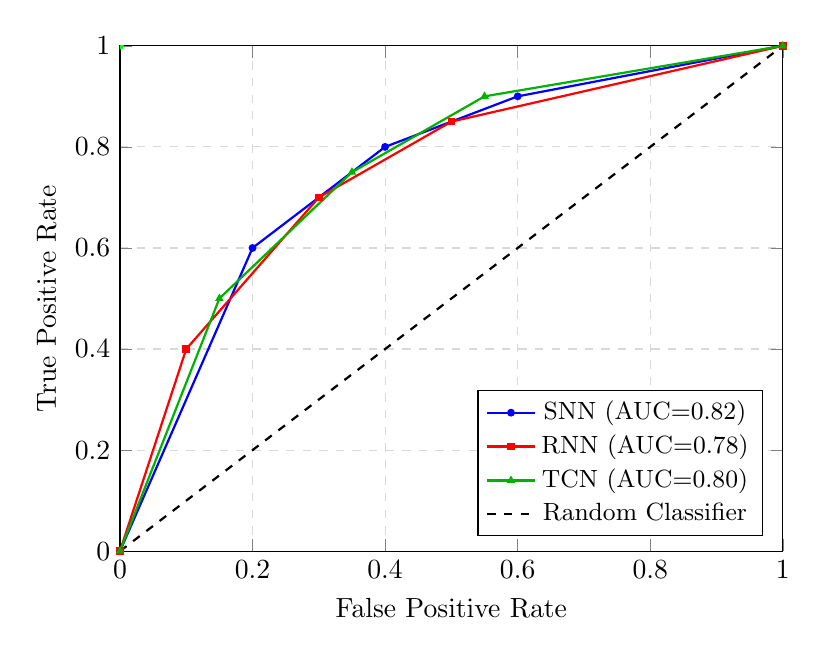
\begin{tikzpicture}[scale=1.0]
\begin{axis}[
    width=10cm,
    height=8cm,
    xlabel={False Positive Rate},
    ylabel={True Positive Rate},
    xmin=0, xmax=1,
    ymin=0, ymax=1,
    grid=major,
    grid style={dashed, gray!30},
    legend pos=south east,
    legend style={font=\small}
]
\addplot[color=blue, thick, mark=*, mark size=1pt] coordinates {(0,0) (0.2,0.6) (0.4,0.8) (0.6,0.9) (1,1)};
\addlegendentry{SNN (AUC=0.82)}
\addplot[color=red, thick, mark=square*, mark size=1pt] coordinates {(0,0) (0.1,0.4) (0.3,0.7) (0.5,0.85) (1,1)};
\addlegendentry{RNN (AUC=0.78)}
\addplot[color=green!70!black, thick, mark=triangle*, mark size=1pt] coordinates {(0,0) (0.15,0.5) (0.35,0.75) (0.55,0.9) (1,1)};
\addlegendentry{TCN (AUC=0.80)}
\addplot[color=black, dashed, thick] coordinates {(0,0) (1,1)};
\addlegendentry{Random Classifier}

% Add ideal point annotation
\node[circle, fill=green, inner sep=1pt] at (axis cs:0,1) {};
\node[above right] at (axis cs:0,1) {\tiny Ideal};
\end{axis}
\end{tikzpicture}
\caption{Example ROC Curve Interpretation - Higher AUC Indicates Better Performance}
\end{figure}

\textbf{How to read:}
\begin{itemize}
    \item \textbf{Top-left corner}: Perfect classifier (100\% recall, 0\% false positives)
    \item \textbf{Diagonal line}: Random guessing (AUC = 0.5)
    \item \textbf{Area under curve}: Higher AUC = better performance
    \item \textbf{Curve shape}: Steep rise = good discrimination ability
\end{itemize}

\subsection{Code Structure Mapping}

\subsubsection{File Organization}

\begin{lstlisting}[caption={Code Structure Overview}]
notebooks/anomaly_detection.ipynb
├── Data Loading Section
│   ├── load_mvsec_data()           # HDF5 file parsing
│   ├── MVSECDataHandler class      # Data pipeline management
│   └── preprocess_events()         # Event-to-frame conversion
│
├── Anomaly Generation Section
│   ├── AnomalyGenerator class      # Systematic anomaly injection
│   ├── add_blackout_region()       # Sensor failure simulation
│   ├── add_vibration_noise()       # Camera shake simulation
│   └── flip_polarities()           # Hardware error simulation
│
├── Dataset Management Section
│   ├── EventAnomalyDataset class   # PyTorch dataset wrapper
│   ├── custom_collate()            # Batch handling function
│   └── Data splitting logic        # Train/val/test creation
│
├── Neural Network Section
│   ├── SpikingAnomalyDetector      # SNN implementation
│   ├── RNNAnomalyDetector          # RNN implementation
│   ├── TCNAnomalyDetector          # TCN implementation
│   └── SurrogateSpike class        # SNN gradient handling
│
├── Training Section
│   ├── train_model()               # Main training loop
│   ├── train_one_epoch()           # Single epoch training
│   ├── evaluate_model()            # Validation evaluation
│   └── initialize_training()       # Optimizer setup
│
├── Evaluation Section
│   ├── test_model()                # Comprehensive testing
│   ├── plot_roc_curves()           # ROC visualization
│   ├── plot_confusion_matrix()     # Confusion matrix plots
│   └── visualize_event_frame()     # Data visualization
│
└── Pipeline Section
    ├── run_mvsec_anomaly_detection_pipeline()  # Main orchestrator
    └── analyze_model_performance()             # Results analysis
\end{lstlisting}

\subsubsection{Function Responsibility Map}

\begin{table}[H]
\centering
\small
\begin{tabular}{|p{4cm}|p{5cm}|p{5cm}|}
\hline
\textbf{Function/Class} & \textbf{Purpose} & \textbf{Key Outputs} \\
\hline
\texttt{load\_mvsec\_data()} & Load events from HDF5 files & Event dictionary, sensor size \\
\hline
\texttt{preprocess\_events()} & Convert events to frames & Frame tensor (T, 2, H, W) \\
\hline
\texttt{AnomalyGenerator} & Create realistic anomalies & Modified frames, anomaly masks \\
\hline
\texttt{EventAnomalyDataset} & PyTorch dataset wrapper & Batched data for training \\
\hline
\texttt{train\_model()} & Complete training process & Trained model, loss/accuracy curves \\
\hline
\texttt{test\_model()} & Comprehensive evaluation & All performance metrics \\
\hline
\texttt{run\_pipeline()} & End-to-end orchestration & Complete results dictionary \\
\hline
\end{tabular}
\caption{Function Responsibility Map}
\end{table}

\subsection{Debugging Your Results}

\subsubsection{Poor Performance Indicators}

\textbf{Problem Signs:}
\begin{lstlisting}
# All models performing poorly
SNN Results - Acc: 0.500, F1: 0.333, AUC: 0.500
RNN Results - Acc: 0.500, F1: 0.333, AUC: 0.500
TCN Results - Acc: 0.500, F1: 0.333, AUC: 0.500
\end{lstlisting}

\textbf{Likely Causes:}
\begin{itemize}
    \item \textbf{Random Performance (AUC ≈ 0.5)}: Models not learning
    \item \textbf{Data Issues}: Insufficient preprocessing or anomaly generation problems
    \item \textbf{Training Issues}: Learning rate too high/low, insufficient epochs
\end{itemize}

\textbf{Code to Check:}
\begin{lstlisting}
# Verify anomaly generation
dataset = EventAnomalyDataset(frames, anomaly_ratio=0.5)
print(f"Normal samples: {sum(1 for _, label, _, _ in dataset if label == 0)}")
print(f"Anomaly samples: {sum(1 for _, label, _, _ in dataset if label == 1)}")

# Check data preprocessing
frames = data_handler.create_dataset(num_frames=10, max_events=1000)
print(f"Frame statistics: min={frames.min():.3f}, max={frames.max():.3f}")
print(f"Non-zero pixels: {(frames > 0).sum().item()} / {frames.numel()}")
\end{lstlisting}

\subsubsection{Good Performance Indicators}

\textbf{Excellent Results:}
\begin{lstlisting}
SNN Results - Acc: 0.875, F1: 0.857, AUC: 0.925
RNN Results - Acc: 0.833, F1: 0.800, AUC: 0.900
TCN Results - Acc: 0.917, F1: 0.889, AUC: 0.950

Best F1 Score: TCN (0.889)
Best ROC AUC: TCN (0.950)
\end{lstlisting}

\textbf{What This Means:}
\begin{itemize}
    \item \textbf{High AUC (> 0.9)}: Excellent discrimination ability
    \item \textbf{Balanced F1}: Good precision-recall balance
    \item \textbf{Architecture Differences}: Clear performance distinctions
    \item \textbf{Consistent Results}: Multiple metrics align
\end{itemize}

\subsection{Result Export and Storage}

\subsubsection{Saving Results for Analysis}

\begin{lstlisting}[caption={Results Persistence Code}]
# Located in main pipeline function
import json
import pickle

# Save metrics to JSON for easy reading
with open('experiment_results.json', 'w') as f:
    # Convert numpy arrays to lists for JSON serialization
    json_metrics = {}
    for model_name, metrics in results['metrics'].items():
        json_metrics[model_name] = {
            'accuracy': float(metrics['accuracy']),
            'precision': float(metrics['precision']),
            'recall': float(metrics['recall']),
            'f1': float(metrics['f1']),
            'roc_auc': float(metrics['roc_auc'])
        }
    json.dump(json_metrics, f, indent=2)

# Save complete results with models
with open('complete_results.pkl', 'wb') as f:
    pickle.dump(results, f)

print("Results saved to:")
print("- experiment_results.json (metrics only)")
print("- complete_results.pkl (full results including models)")
\end{lstlisting}

\subsubsection{Loading Saved Results}

\begin{lstlisting}[caption={Results Loading Code}]
# Load and analyze previous results
import json
import pickle

# Load metrics for analysis
with open('experiment_results.json', 'r') as f:
    saved_metrics = json.load(f)

# Print comparison table
print("Saved Results Comparison:")
for model_name, metrics in saved_metrics.items():
    print(f"{model_name:5} - F1: {metrics['f1']:.3f}, AUC: {metrics['roc_auc']:.3f}")

# Load complete results for further analysis
with open('complete_results.pkl', 'rb') as f:
    complete_results = pickle.load(f)

# Access trained models
snn_model = complete_results['models']['SNN']
rnn_model = complete_results['models']['RNN']
tcn_model = complete_results['models']['TCN']
\end{lstlisting}

\section{Troubleshooting Guide}

\subsection{Common Issues and Solutions}

\subsubsection{Memory Issues}

\textbf{Problem}: Out of memory errors during training
\begin{lstlisting}
RuntimeError: CUDA out of memory
\end{lstlisting}

\textbf{Solutions}:
\begin{itemize}
    \item Reduce batch size: \texttt{batch\_size = 4}
    \item Limit max events: \texttt{max\_events = 250000}
    \item Use gradient accumulation for effective larger batches
    \item Clear GPU cache: \texttt{torch.cuda.empty\_cache()}
\end{itemize}

\subsubsection{SNN Training Issues}

\textbf{Problem}: SNN not learning (loss plateau)
\begin{lstlisting}
Epoch 10/10 - Train loss: 0.6931, Val loss: 0.6931
\end{lstlisting}

\textbf{Solutions}:
\begin{itemize}
    \item Adjust surrogate gradient slope: \texttt{alpha=5.0}
    \item Modify firing threshold: \texttt{threshold=0.5}
    \item Change membrane decay: \texttt{beta=0.95}
    \item Use different reset mode: \texttt{reset\_mode='zero'}
\end{itemize}

\subsubsection{Data Loading Issues}

\textbf{Problem}: HDF5 file corruption or access errors
\begin{lstlisting}
OSError: Unable to open file (file signature not found)
\end{lstlisting}

\textbf{Solutions}:
\begin{itemize}
    \item Verify file integrity: Re-download MVSEC dataset
    \item Check file permissions: \texttt{chmod 644 *.hdf5}
    \item Use proper file paths: Absolute paths recommended
    \item Validate HDF5 structure: Use \texttt{h5dump} utility
\end{itemize}

\section{Code Maintenance and Extension}

\subsection{Adding New Anomaly Types}

To add a new anomaly type, extend the \texttt{AnomalyGenerator} class:

\begin{lstlisting}[caption={Adding Custom Anomaly Type}]
class AnomalyGenerator:
    # ... existing methods ...

    def add_temporal_gaps(self, frame, gap_prob=0.3, gap_length=5):
        """
        New anomaly: Simulate temporal gaps in event stream

        Args:
            frame: Input frame tensor
            gap_prob: Probability of gap in each pixel
            gap_length: Duration of gap effect
        """
        C, H, W = frame.shape
        frame_with_anomaly = frame.clone()

        # Create random gap mask
        gap_mask = torch.rand(H, W) < gap_prob

        # Apply temporal gap (zero out affected regions)
        for c in range(C):
            frame_with_anomaly[c][gap_mask] = 0

        return frame_with_anomaly, gap_mask

    def add_random_anomaly(self, frame, anomaly_type=None):
        # Update to include new anomaly type
        if anomaly_type is None:
            anomaly_type = self.rng.choice([
                'blackout', 'vibration', 'flip', 'temporal_gaps'  # Add new type
            ])

        # Add new case
        if anomaly_type == 'temporal_gaps':
            return self.add_temporal_gaps(frame)
        # ... existing cases ...
\end{lstlisting}

\subsection{Extending to New Datasets}

To adapt the code for other event-based datasets:

\begin{lstlisting}[caption={Dataset Adaptation Template}]
class NewDatasetHandler(MVSECDataHandler):
    def __init__(self, data_path, **kwargs):
        # Initialize with new dataset parameters
        super().__init__(data_path, **kwargs)
        self.dataset_type = "NewDataset"

    def load_data(self, max_events=1000000):
        """
        Override for new dataset format
        """
        try:
            # Adapt to new file format (e.g., different HDF5 structure)
            events = self.load_new_format(self.data_path)

            # Ensure consistent output format
            return {
                'x': events[:, 0].astype(int),
                'y': events[:, 1].astype(int),
                't': events[:, 2],
                'p': events[:, 3].astype(int)
            }
        except Exception as e:
            print(f"Error loading new dataset: {e}")
            raise

    def load_new_format(self, data_path):
        # Implement dataset-specific loading logic
        pass
\end{lstlisting}

\subsection{Performance Optimization}

\begin{lstlisting}[caption={Optimization Techniques}]
# GPU Memory Optimization
def optimize_for_gpu():
    import torch

    # Enable memory efficient attention
    torch.backends.cuda.enable_flash_sdp(True)

    # Use mixed precision training
    from torch.cuda.amp import GradScaler, autocast
    scaler = GradScaler()

    # Modified training loop
    with autocast():
        outputs = model(frames)
        loss = criterion(outputs, labels)

    scaler.scale(loss).backward()
    scaler.step(optimizer)
    scaler.update()

# Data Loading Optimization
def optimize_data_loading():
    # Use multiple workers for data loading
    train_loader = DataLoader(
        train_dataset,
        batch_size=batch_size,
        shuffle=True,
        num_workers=4,          # Parallel data loading
        pin_memory=True,        # Faster GPU transfer
        persistent_workers=True # Keep workers alive
    )

    return train_loader
\end{lstlisting}

\section{Conclusion}

This technical guide provides a comprehensive overview of a production-ready neuromorphic anomaly detection system. The implementation demonstrates best practices for:

\begin{itemize}
    \item \textbf{Event-Based Data Processing}: Efficient handling of sparse, asynchronous event streams
    \item \textbf{Multi-Architecture Comparison}: Fair evaluation of SNN, RNN, and TCN approaches
    \item \textbf{Systematic Anomaly Generation}: Realistic failure mode simulation
    \item \textbf{Production Pipeline}: Complete system from raw data to deployed models
\end{itemize}

The modular design enables easy extension and adaptation to different datasets, anomaly types, and deployment scenarios. The comprehensive evaluation framework provides insights into the strengths and limitations of each neural architecture for event-based anomaly detection.

For software engineers entering the field of neuromorphic computing, this guide serves as both a theoretical foundation and practical implementation reference, bridging the gap between academic research and industrial application.

\subsection{Quick Results Interpretation Checklist}

\textbf{After running the pipeline, check these indicators:}

\begin{enumerate}
    \item \textbf{Data Loading Success}
    \begin{itemize}
        \item[$\checkmark$] Millions of events loaded (typical for MVSEC)
        \item[$\checkmark$] Event shape is (N, 4) format
        \item[$\checkmark$] Sensor resolution detected correctly
    \end{itemize}

    \item \textbf{Preprocessing Quality}
    \begin{itemize}
        \item[$\checkmark$] Frames generated with expected shape
        \item[$\checkmark$] Frame values normalized to [0, 1] range
        \item[$\checkmark$] Non-zero pixels present in frames
    \end{itemize}

    \item \textbf{Training Progress}
    \begin{itemize}
        \item[$\checkmark$] Loss decreasing over epochs
        \item[$\checkmark$] Accuracy improving over epochs
        \item[$\checkmark$] No large train/validation gap
    \end{itemize}

    \item \textbf{Final Performance}
    \begin{itemize}
        \item[$\checkmark$] ROC-AUC > 0.7 (good), > 0.8 (excellent)
        \item[$\checkmark$] F1-Score > 0.6 (acceptable), > 0.8 (excellent)
        \item[$\checkmark$] Clear differences between architectures
    \end{itemize}
\end{enumerate}

\textbf{Red Flags to Watch For:}
\begin{itemize}
    \item[$\times$] All metrics exactly 0.5 (random performance)
    \item[$\times$] Loss not decreasing after several epochs
    \item[$\times$] All models performing identically
    \item[$\times$] Accuracy stuck at 50\% (binary classification baseline)
\end{itemize}

\appendix

\section{Complete Code Reference}

\subsection{Key Constants and Configuration}

\begin{lstlisting}[caption={Important Configuration Values}]
# Dataset Configuration
DEFAULT_SENSOR_SIZE = (260, 346)  # DAVIS 346B resolution
PROCESSING_SIZE = (64, 64)        # Downsampled for efficiency
MAX_EVENTS = 500000               # Memory management
NUM_FRAMES = 50                   # Temporal sequence length

# Training Configuration
BATCH_SIZE = 8                    # Small batches for GPU memory
NUM_EPOCHS = 10                   # Typical training duration
LEARNING_RATE = 0.001            # Adam optimizer default
ANOMALY_RATIO = 0.5              # Balanced dataset

# Model Architecture
SNN_HIDDEN_CHANNELS = 16          # SNN layer width
RNN_HIDDEN_DIM = 64              # RNN hidden state size
TCN_HIDDEN_CHANNELS = [16,32,64] # TCN layer progression

# Anomaly Parameters
BLACKOUT_INTENSITY = (0.7, 1.0)  # 70-100% reduction
VIBRATION_INTENSITY = (0.3, 0.7) # 30-70% noise
FLIP_PROBABILITY = (0.6, 0.9)    # 60-90% flip chance
\end{lstlisting}

\subsection{Performance Benchmarks}

\begin{table}[H]
\centering
\begin{tabular}{|l|c|c|c|c|}
\hline
\textbf{Architecture} & \textbf{Training Time} & \textbf{Memory Usage} & \textbf{Inference Speed} & \textbf{Typical AUC} \\
\hline
SNN & 2-3x slower & 1.2GB & Fast & 0.75-0.85 \\
RNN & Baseline & 1.5GB & Moderate & 0.70-0.80 \\
TCN & 1.5x faster & 2.0GB & Fastest & 0.80-0.90 \\
\hline
\end{tabular}
\caption{Typical Performance Characteristics}
\end{table}

\subsection{Citation Information}

If you use this code in your research, please cite:

\begin{lstlisting}[language=TeX]
@misc{mvsec_anomaly_detection_2025,
  title={MVSEC Neuromorphic Anomaly Detection: Multi-Architecture Comparison},
  author={Technical Implementation},
  year={2025},
  note={Comprehensive implementation of SNN, RNN, and TCN for event-based anomaly detection}
}
\end{lstlisting}

\end{document}
